
%(BEGIN_QUESTION)
% Copyright 2014, Tony R. Kuphaldt, released under the Creative Commons Attribution License (v 1.0)
% This means you may do almost anything with this work of mine, so long as you give me proper credit

Calculate all voltages and all currents in this transformer circuit, assuming the 3.3 k$\Omega$ resistor drops 40 volts:

$$\includegraphics[width=15.5cm]{i01271x01.eps}$$

\begin{itemize}
\item{} $V_{source}$ = 
\item{} $V_{primary}$ = 
\item{} $V_{secondary}$ = 
\item{} $I_{source}$ =  
\item{} $I_{primary}$ = 
\item{} $I_{secondary}$ = 
\end{itemize}

\underbar{file i01271}
%(END_QUESTION)





%(BEGIN_ANSWER)

\begin{itemize}
\item{} $V_{source}$ = 18.84 V
\item{} $V_{primary}$ = 18.84 V
\item{} $V_{secondary}$ = 46.06 V
\item{} $I_{source}$ = 76.74 mA
\item{} $I_{primary}$ = 29.63 mA
\item{} $I_{secondary}$ = 12.12 mA
\end{itemize}

%(END_ANSWER)





%(BEGIN_NOTES)

Most transformer problems are nothing more than ratios, but some students find ratios difficult to handle.  Questions such as this are great for having students come up to the board in the front of the classroom and demonstrating how they obtained the results.

%INDEX% Electronics review: transformer ratios

%(END_NOTES)


